\documentclass[11pt, a4paper]{article}

\usepackage[utf8]{inputenc}
\usepackage[T1]{fontenc}
\usepackage[charter]{mathdesign} % Elegant, readable font
\usepackage{geometry}
\geometry{margin=1in}
\usepackage{enumitem}
\usepackage{amsmath}
\usepackage{booktabs}
\usepackage{hyperref}
\usepackage{graphicx} % Required for inserting images (put this in your preamble)
\usepackage{subfig}


\makeatletter
\renewcommand{\maketitle}{
  \begin{flushleft}
    {\huge \textbf{\@title} \par}
    \vspace{0.5cm}
    {\large \@author \par}
    \vspace{0.2cm}
    {\@date \par}
    \vspace{0.2cm}
    \hrule
  \end{flushleft}
}
\makeatother

\title{\LARGE\textbf{Parallel Seam Carving using OpenMP} \\[-0.2em]
    \large Assignment 1 --- High Performance Computing}
\author{
    Plabon Shaha and Guillem Masdemont \\ 
    \small University of Ljubljana, Spring Semester, EMAI Cohort 25--27 
}

\begin{document}

\maketitle

\begin{enumerate}[label={\textbf{Exercise \arabic*:}}]
  \item Execution times are measured for the five resolutions using 1, 2, 4, 8, 16, and 32 threads. We remove 128 seams and average timings across 5 experiments. Performance is evaluated via speed-up, defined as $S = \frac{t_s}{t_p}$, where $t_s$ is the sequential runtime and $t_p$ is the parallel runtime. The results are presented in figure \ref{fig:fixed_cores_performance} for a $4$ core test: 

\begin{figure}[h]
      \centering
      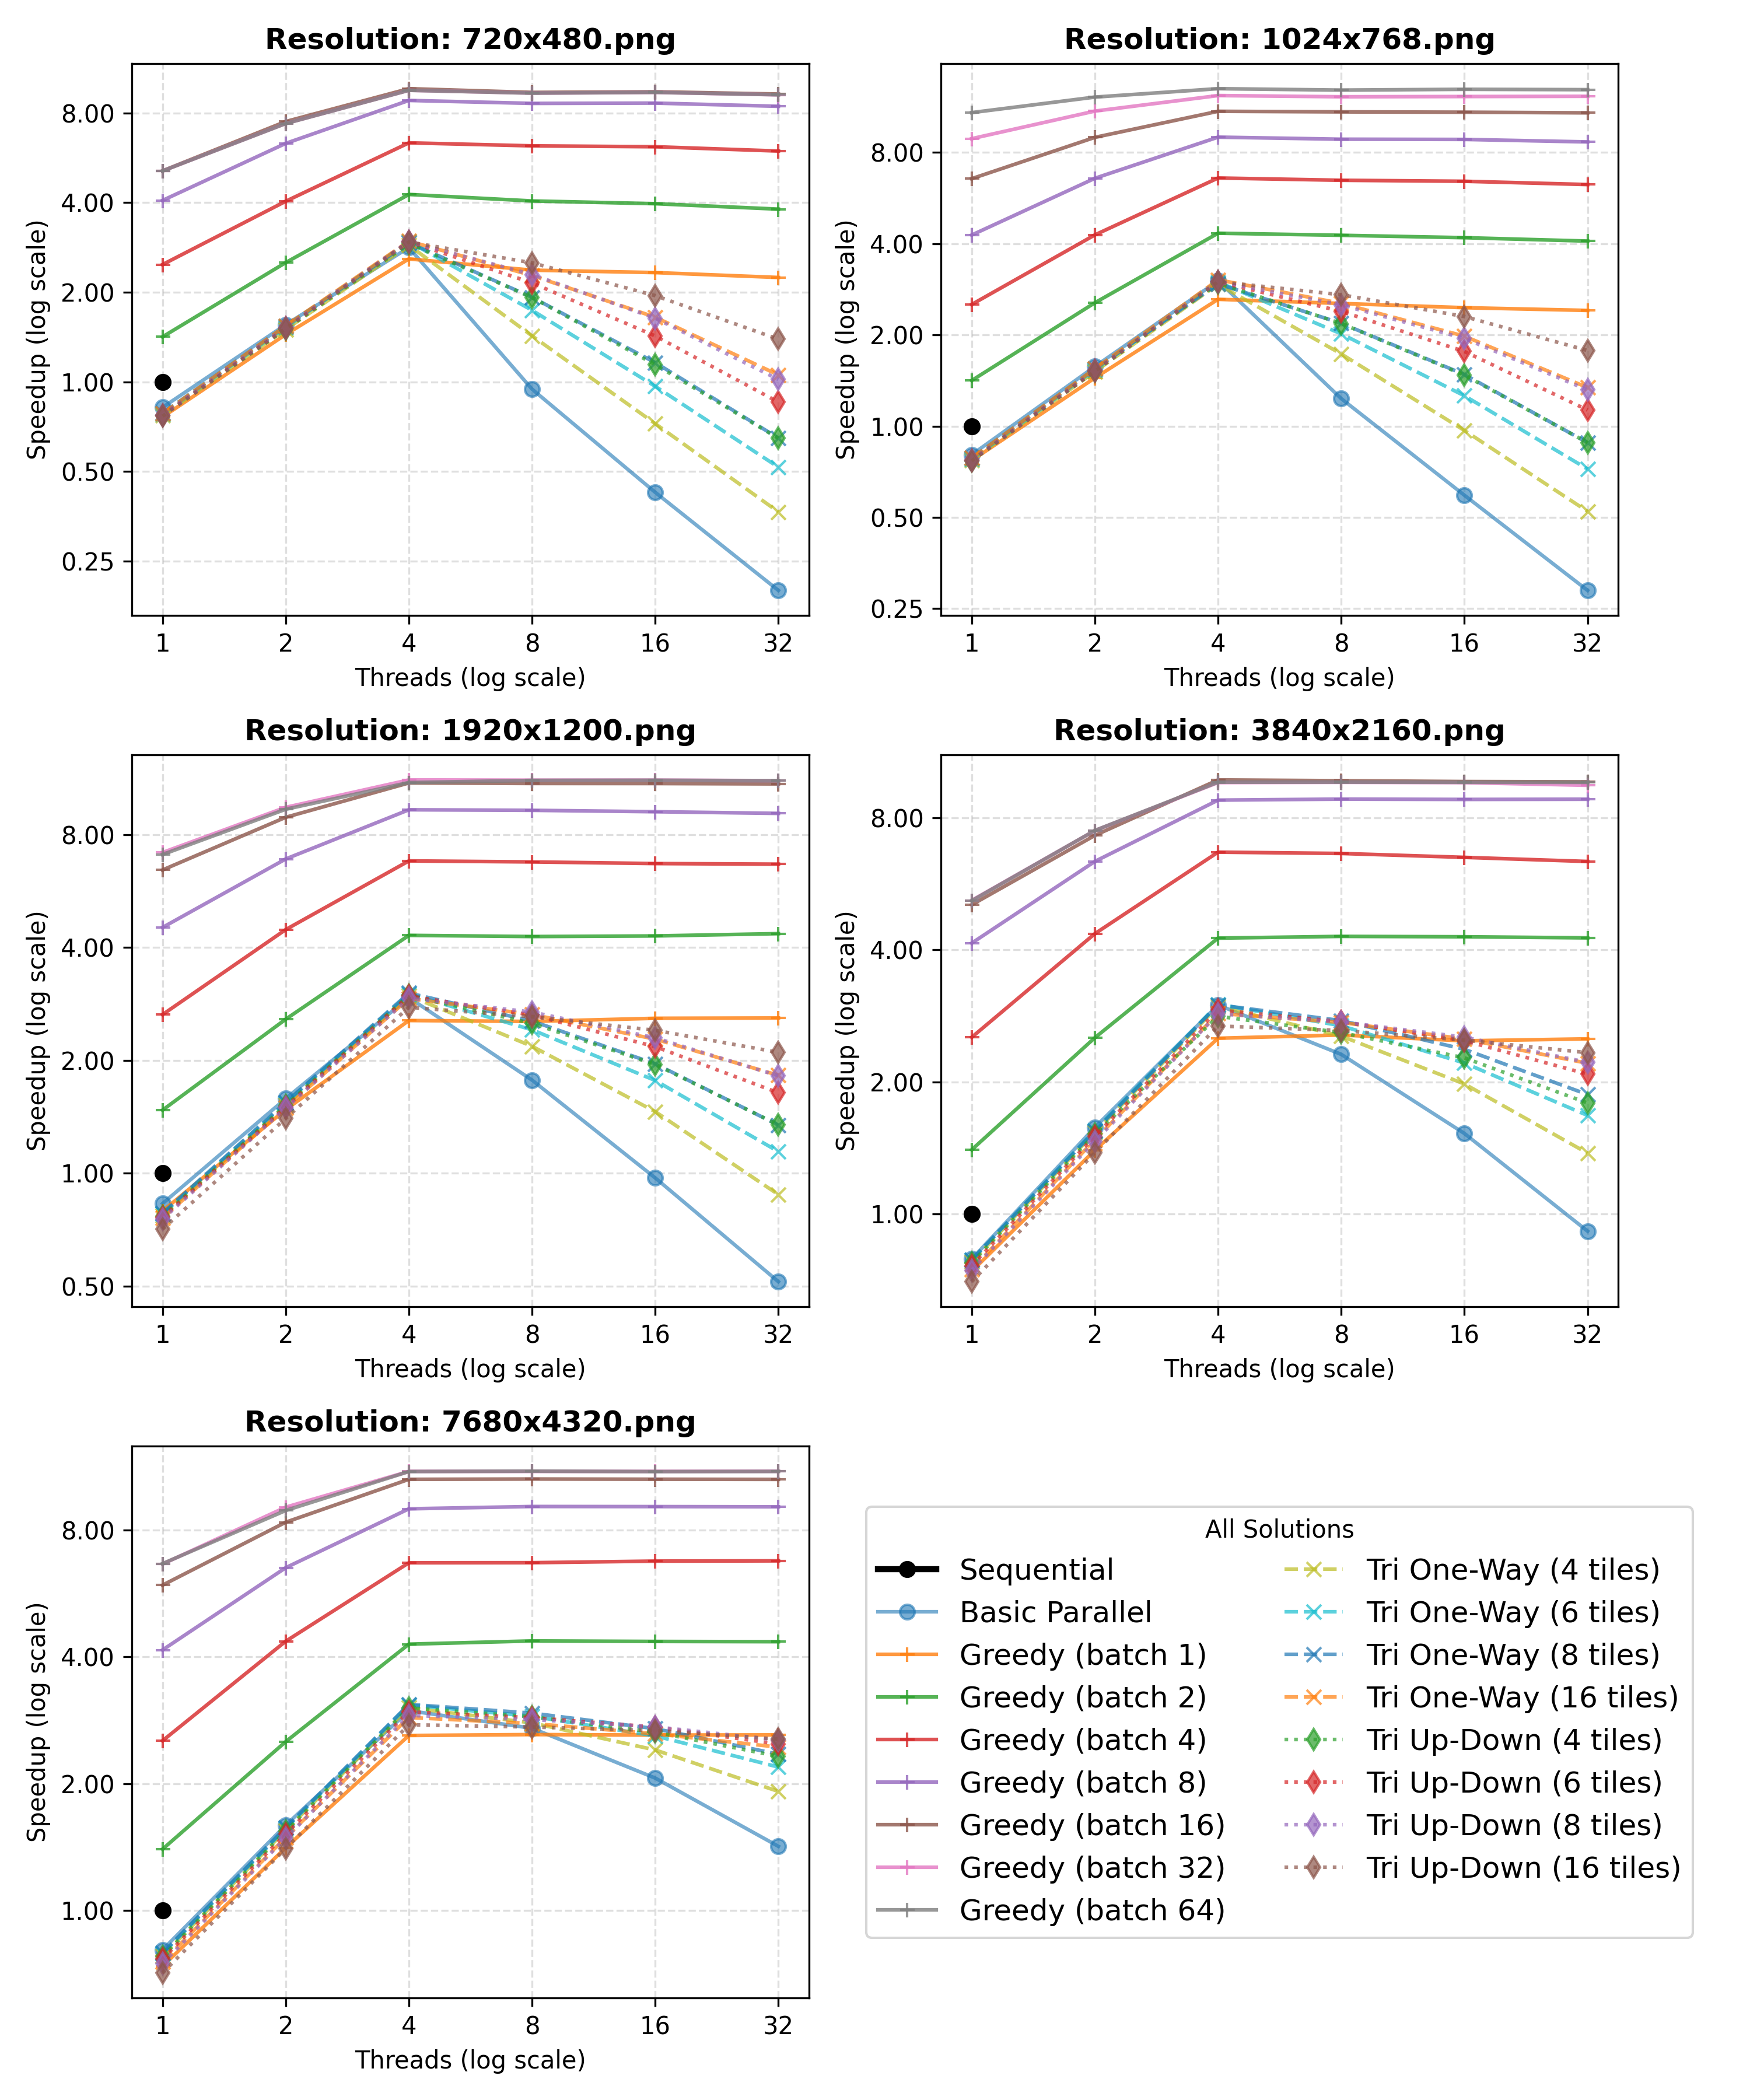
\includegraphics[width=0.85\textwidth]{./images/performance_comprehensive_greedy.png}
      \caption{Speedup analysis for various parallel strategies across five image resolutions. Case use of 4 cores.}
      \label{fig:fixed_cores_performance}
\end{figure}

The following conclusions are drawn: 
\begin{enumerate}

  \item The best performance is typically obtained when the number of OpenMP threads matches the number of physical cores. In this regime, each thread can run on a core without oversubscription, minimizing context switching and scheduling overhead. For this workload, which is strongly memory-access intensive (large matrix traversals and frequent neighborhood reads), adding extra software threads beyond the core count does not increase effective memory bandwidth and may increase cache and memory-system contention. Therefore, oversubscription degrades performance. Figure \ref{fig:fixed_cores_performance} shows this behavior consistently across all parallel tasks, with qualitatively similar trends for $2$, $8$, and $16$ cores. 
  
  \item There is an approximately linear relationship between the number of threads and the achieved speedup, provided the thread count does not exceed the number of physical cores. The parallel efficiency is slightly higher for larger images because the ratio of computation to synchronization overhead improves, and hence there is a more uniform distribution of tasks. 
  
  \item Greddy seam removal performs better than other parallel strategies because we are bypassing several cumulative energy recalculations. Note that performing greedy seam removal is an approximation of the algorithm that may fail. A documented example of this trade-off is provided by \href {https://capstone.cs.ucsb.edu/team_docs_12/ngor_ts.pdf}{Ngor et al.}, where GPU acceleration dramatically reduces execution time at the expense of global optimality.
  
  \item The performance of the triangular approach and the basic row-parallel method remains comparable when the thread count is less than or equal to the core count. In this regime, both strategies distribute an equivalent pixel-processing load per thread, and the hardware can accommodate them properly. However, once the number of threads exceeds the number of physical cores, the triangular approach becomes a superior alternative because it present a reduced frequency of thread re-scheduling. When threads exceed cores, the threads compete to get allocated in the CPU, increasing the computation time.
\end{enumerate}

We present now how the performance behaviour changes as a function of the cores: 
\begin{figure}[h]
      \centering
      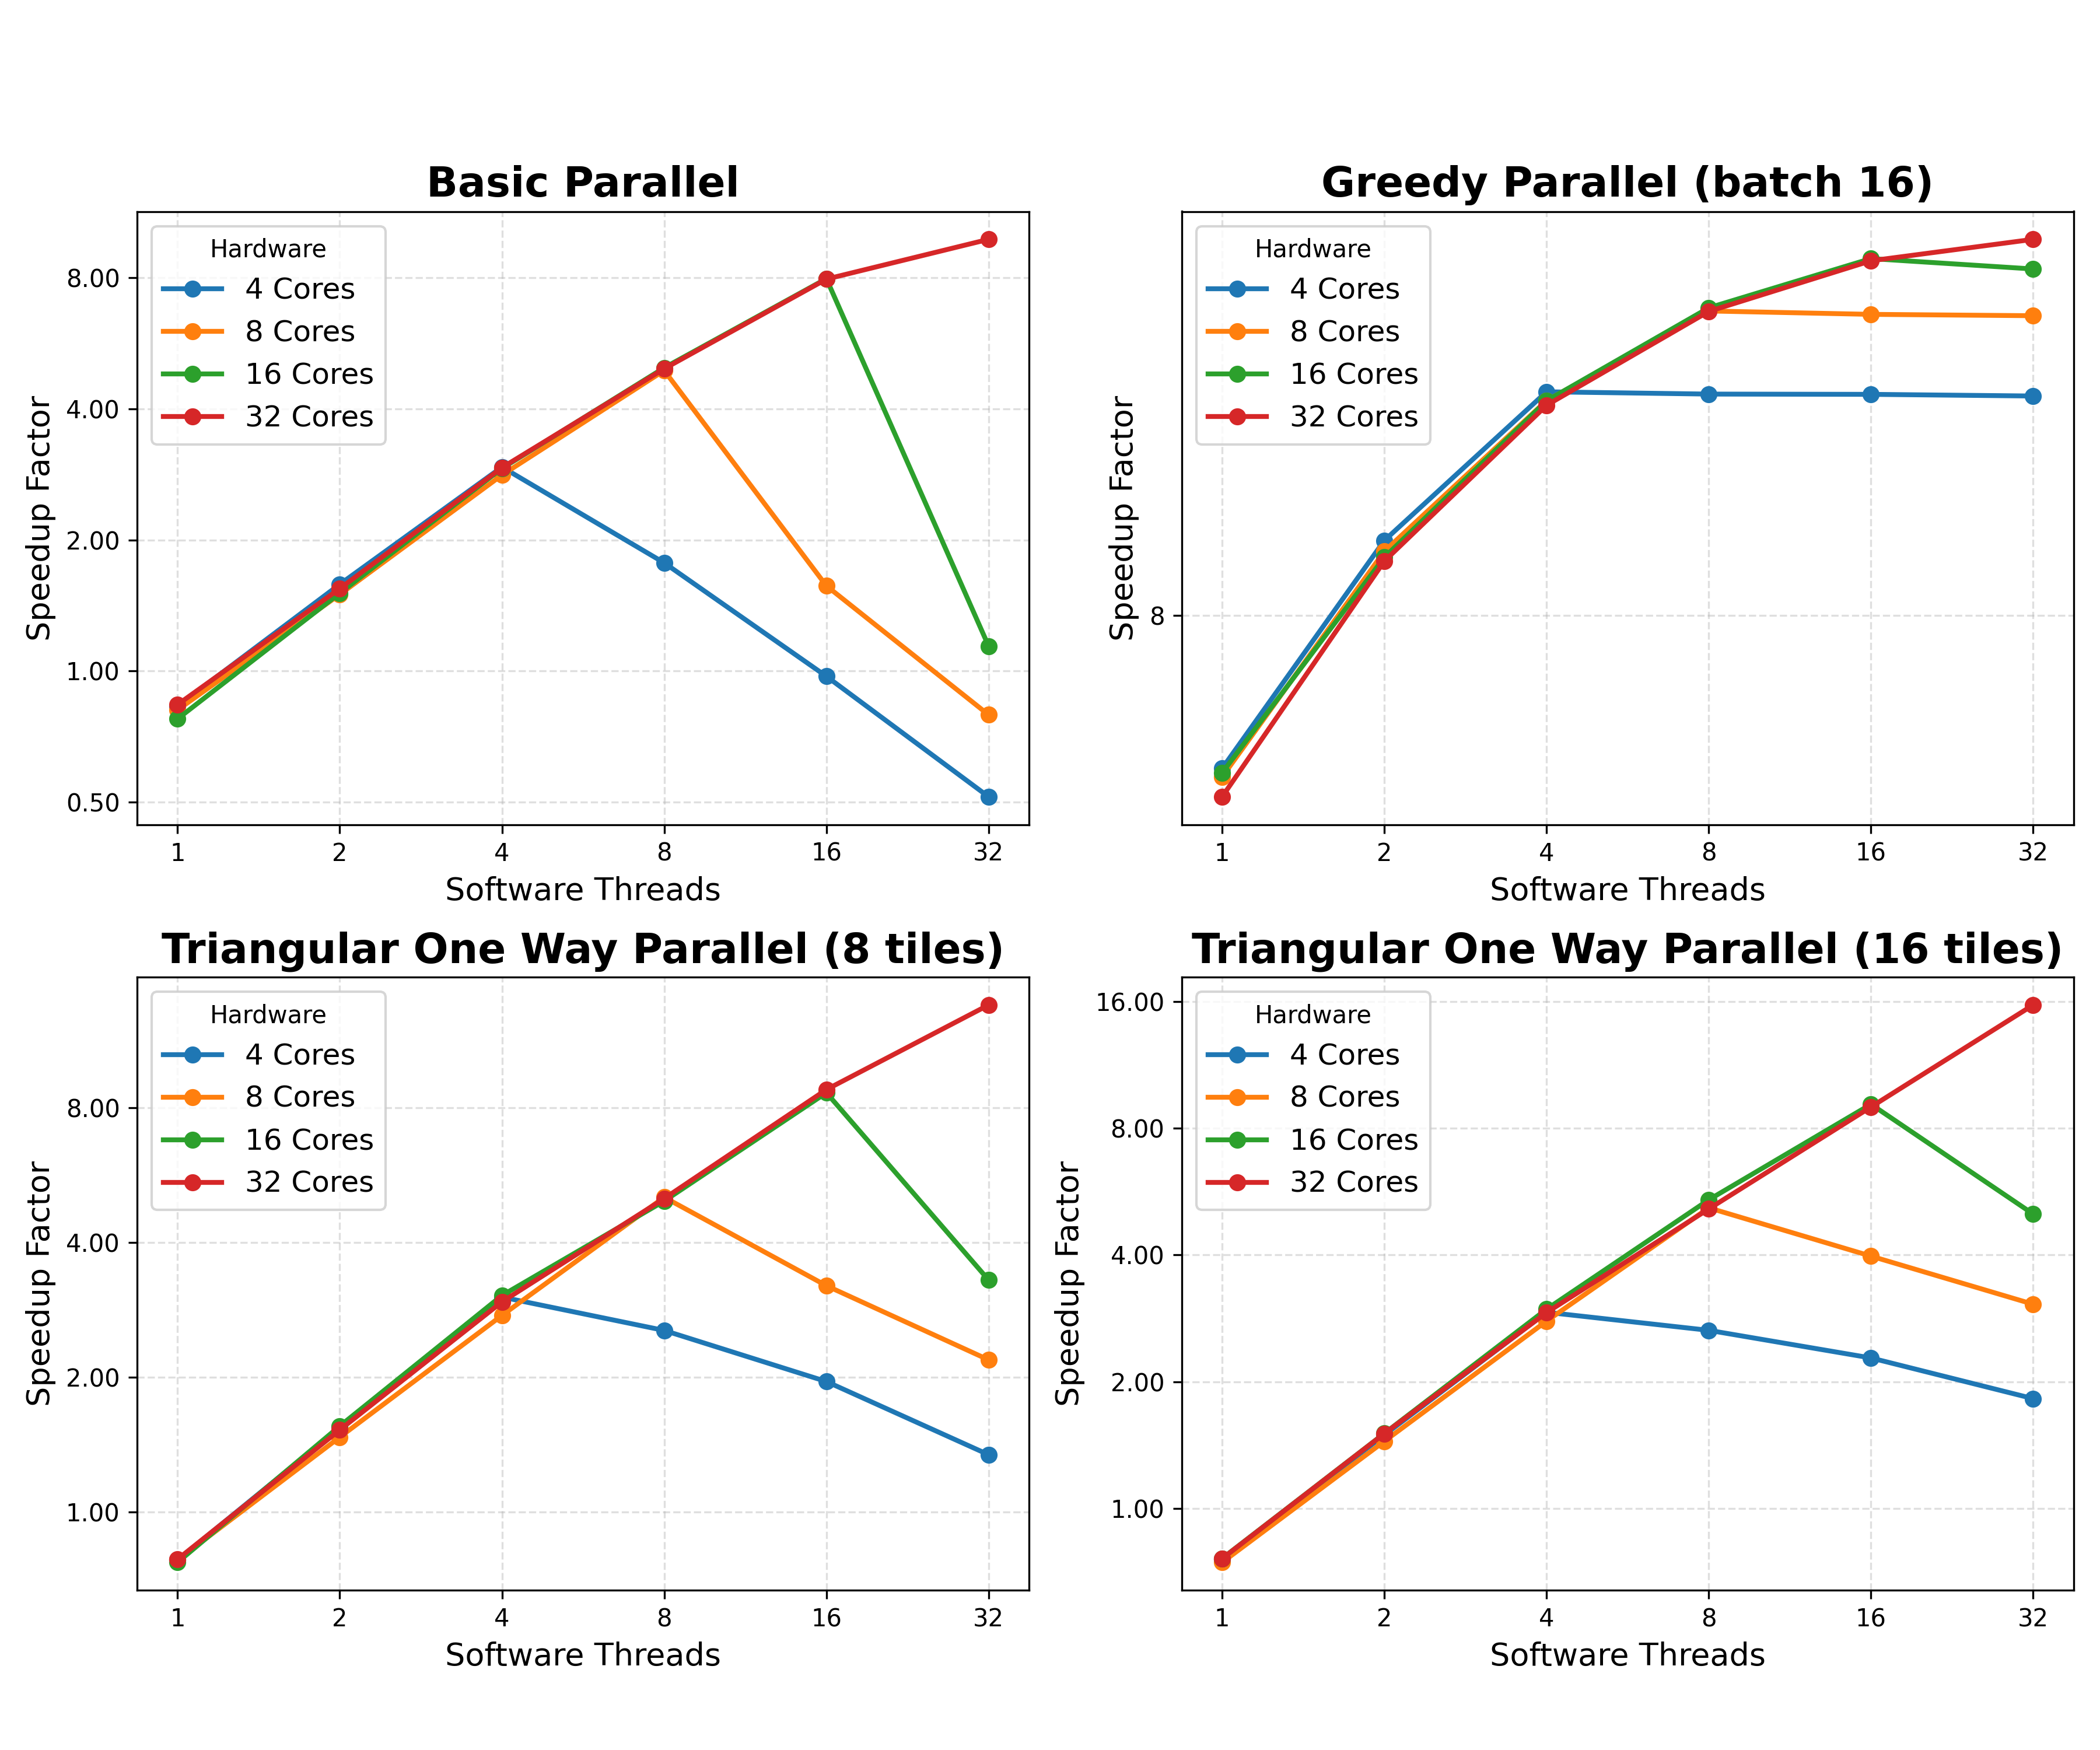
\includegraphics[width=0.75\textwidth]{./images/comparison_by_cores_1920x1200.png}
      \caption{Hardware scalability comparison for the 1920x1200 resolution image.}
      \label{fig:cores_comparison_1920}
\end{figure}

\begin{enumerate}
  \item Across all parallel implementations, we observe that increasing the thread count yields a corresponding increase in speedup within the undersubscribed regime (where threads $\le$ cores). However, once the number of threads surpasses the physical core count, performance degrades due to oversubscription. Consequently, the number of available physical cores represents the practical upper bound for the algorithm's performance. 

\end{enumerate}



\item 

\begin{enumerate}

\item We compare standard seam removal and greedy seam removal across different images and different number of seams to remove. We observe that the algorithm is robust in the dataset, and doesn't present major differences for even seams $500$ seams removed. As shown in figure \ref{fig:four_images_comparison}.  
  

\begin{figure}[h]
    \centering
    \subfloat[\centering ]{{
\includegraphics[width=2.0cm]{../sample_code/parallel_out.png} }}%
    \subfloat[\centering ]{{
\includegraphics[width=2.0cm]{../sample_code/greedy_out.png} }}%
    \subfloat[\centering ]{{
\includegraphics[width=3.2cm]{../sample_code/parallel_out_son_goku_1000.png} }}%
    \subfloat[\centering ]{{
\includegraphics[width=3.2cm]{../sample_code/greedy_out_son_goku_1000.png} }}%
    \caption{Comparison of four seam removal results: alternating between optimized parallel and greedy approaches.}%
    \label{fig:four_images_comparison}%
\end{figure}

\item We present the heuristics found for the number of threads as a function of height, width and core number. 

\begin{itemize}
    \item Thread Allocation heuristic: For high-resolution images ($1024 \times 768$ pixels and above), the optimal thread count is $T = C$, as the high computational density offsets the overhead required to create and synchronize threads (see Figure \ref{fig:fixed_cores_performance}). However, for low-resolution images, peak performance is achieved when $T < C$. In these cases, the latency of thread management exceeds the execution time of the actual workload.

    \begin{figure}[h]
      \centering
      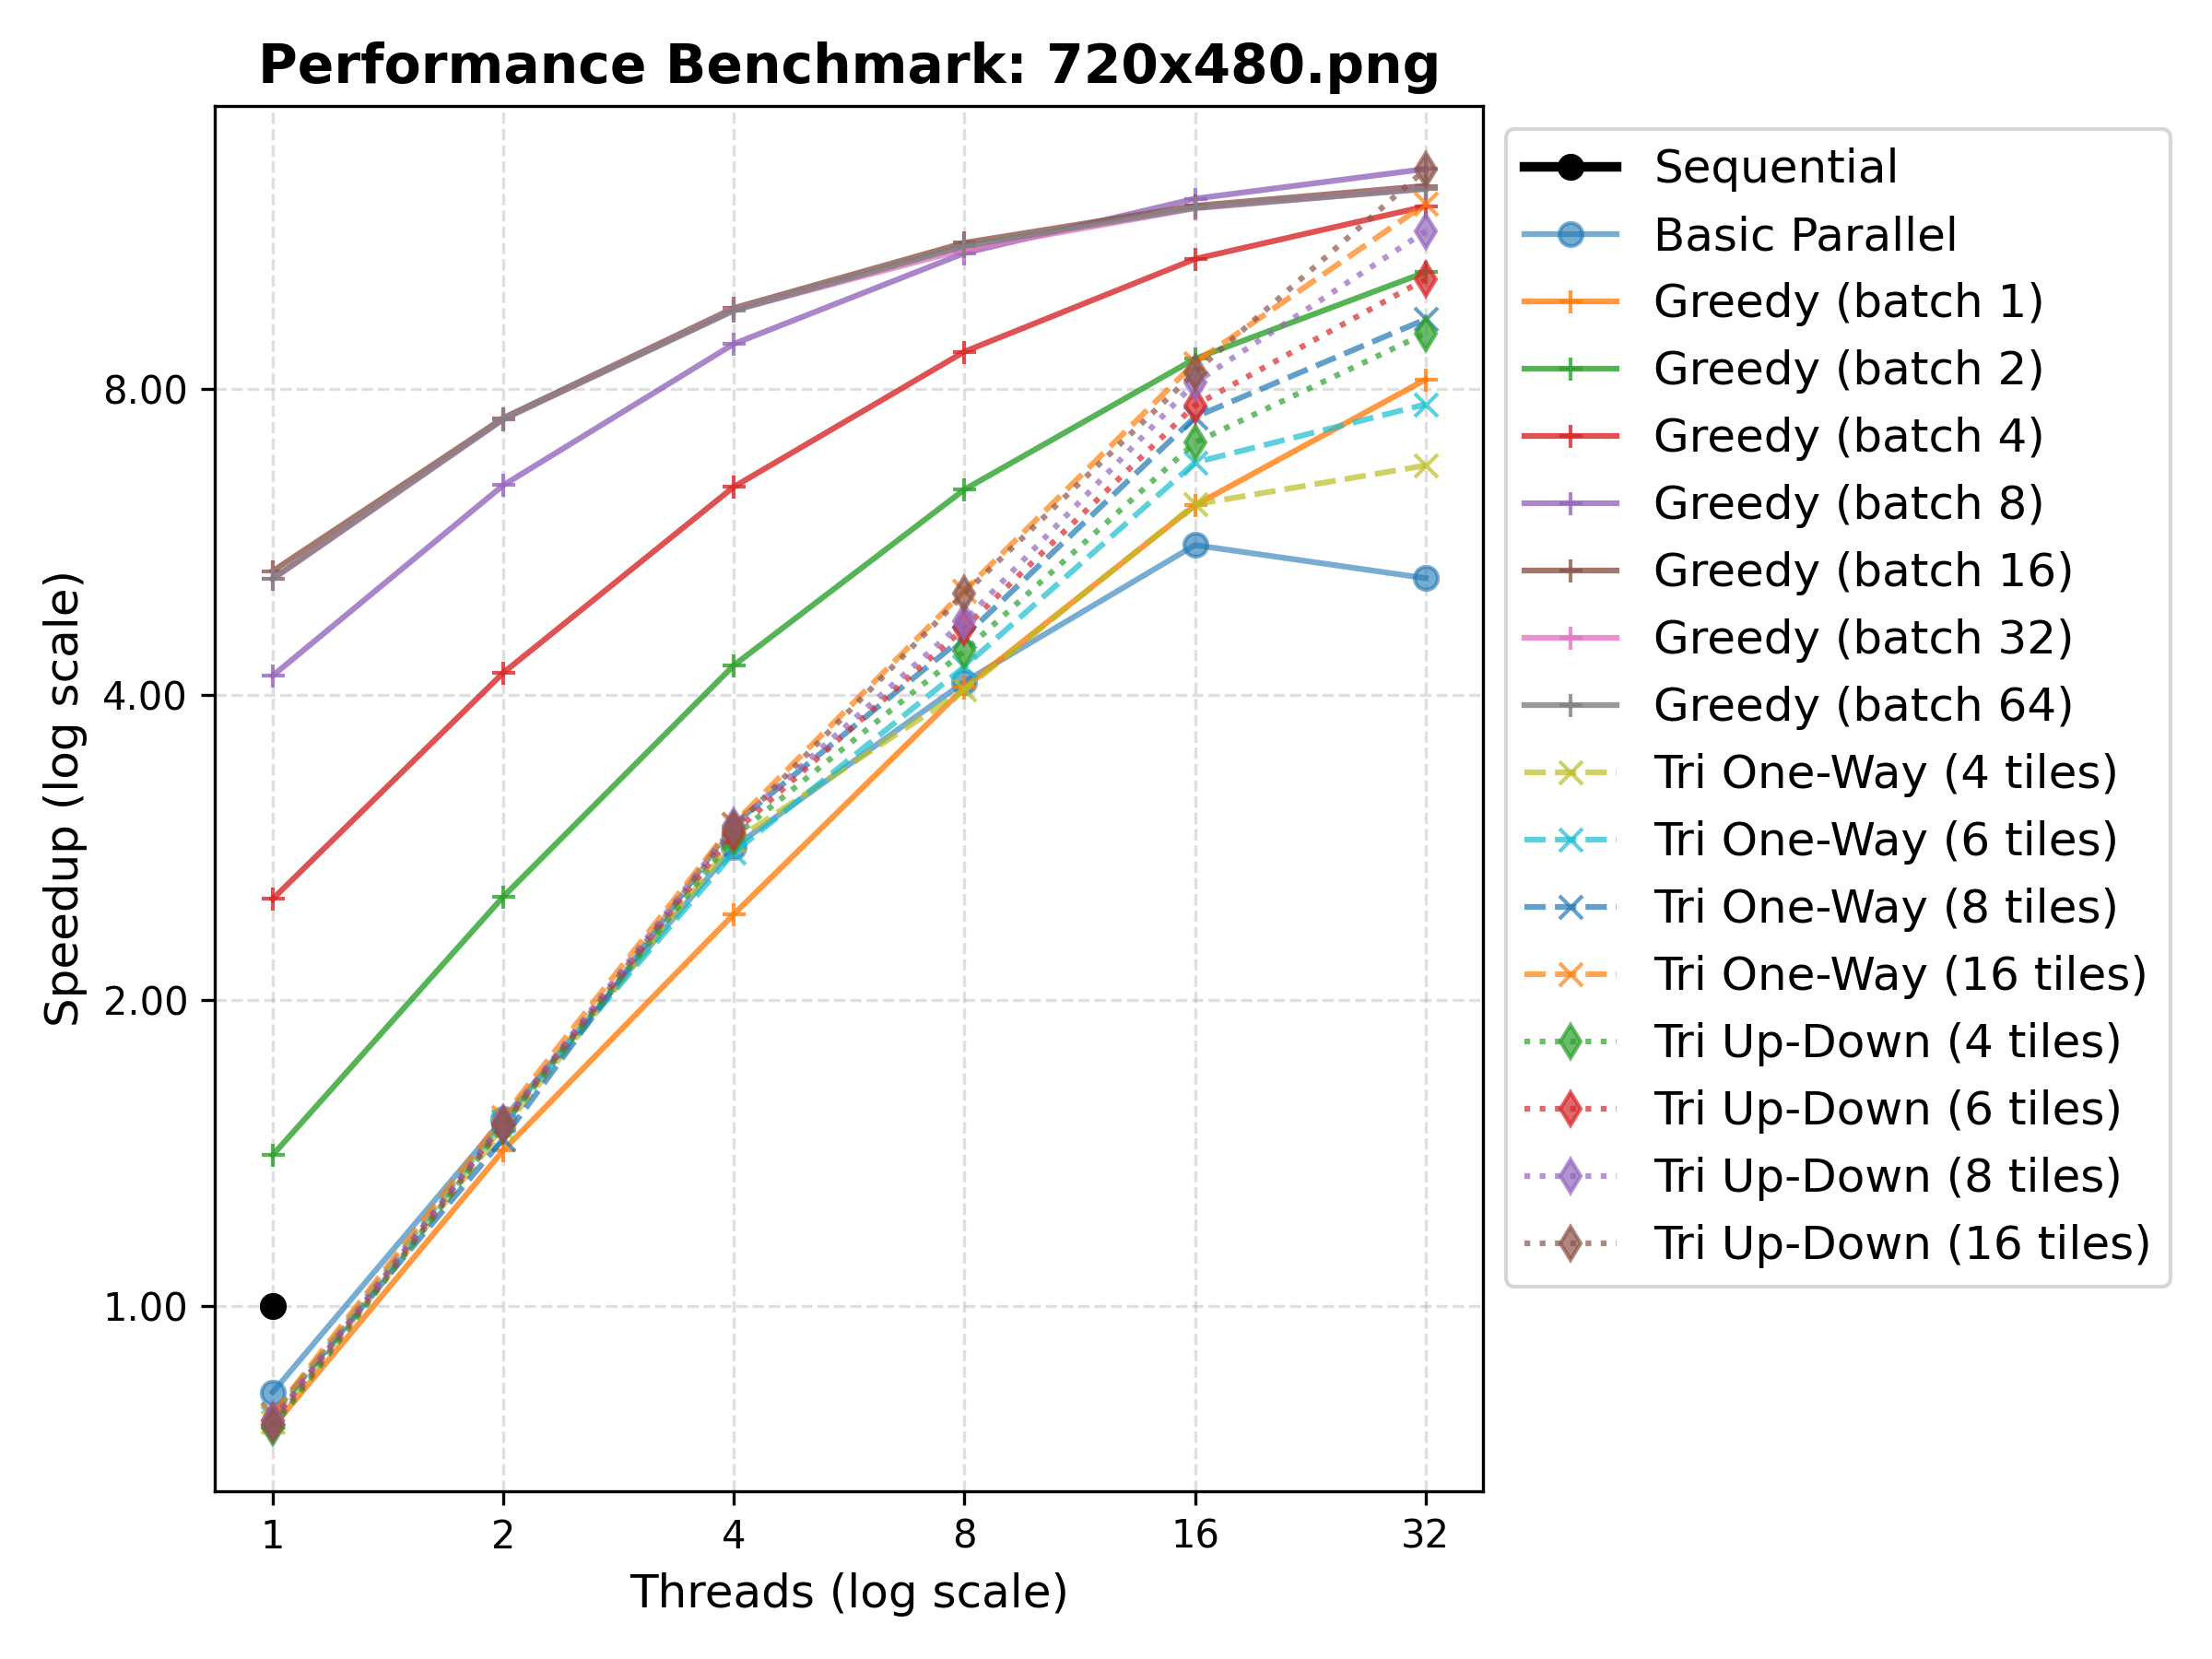
\includegraphics[width=0.5\textwidth]{./images/performance_first_image.png} 
      \caption{Speed up performance for the first image as a function of the number of threads. }
      \label{fig:firstimage} 
    \end{figure}

    Hence we define the heuristic: 
    \begin{equation}
        T(W, H, C) = \min\left(C, \left\lfloor \frac{W \times H \times C}{G} \right\rfloor\right) \quad G = 1024 \times 768 \times 32
    \end{equation}

    Here $G$ is a granularity coefficient we have fine-tuned based on the results observed in Figure \ref{fig:firstimage}. In practice, we should take the closest power of $2$ for the thread number. 
    \\

    We also note that the hardware Numa architecture might play a role here, as the total number of CPU cores it presents is $16$. 

    \item Tile Height Heuristic: In the triangular/wavefront approach, the tile height should be tuned to fit the L2 cache size. This ensures that image computation is large enough to keep all cores busy while remaining small enough to minimize the latency of data storage\footnote{We observe that an alternative heuristic used is $\sqrt{H}$, although we could not verify empirically the validity of it.}.
    \begin{equation}
        h_{tile} \approx \frac{\text{L2 Cache Size (bytes)}}{W \times \text{Bytes per Pixel}}
    \end{equation}
    
\end{itemize}

\item To optimize the seam selection process, we modified the aforementioned traditional dynamic programming approach by implementing a bidirectional energy accumulation. 

The image is bisected at $\bar{y} = \lceil h/2 \rceil$, we execute the parallel triangular approach in parallel, on starting on the top and the other on the bottom as shown in image \ref{fig:midpoint_sync}. The final seam is reconstructed by identifying the optimal midpoint $\hat{x}$ via the formula 
\begin{equation}
  \hat{x} = \underset{i}{\operatorname{argmin}} \left( E(x_i, \bar{y}) + \min \left( E(x_{i-1}, \bar{y}), E(x_i, \bar{y}), E(x_{i+1}, \bar{y}) \right) \right)
\end{equation}
and performing two simultaneous tracebacks, one moving upward and one moving downward from the select $\hat{x}$. 

\begin{figure}[h]
    \centering
    \subfloat[\centering Midpoint Synchronization]{{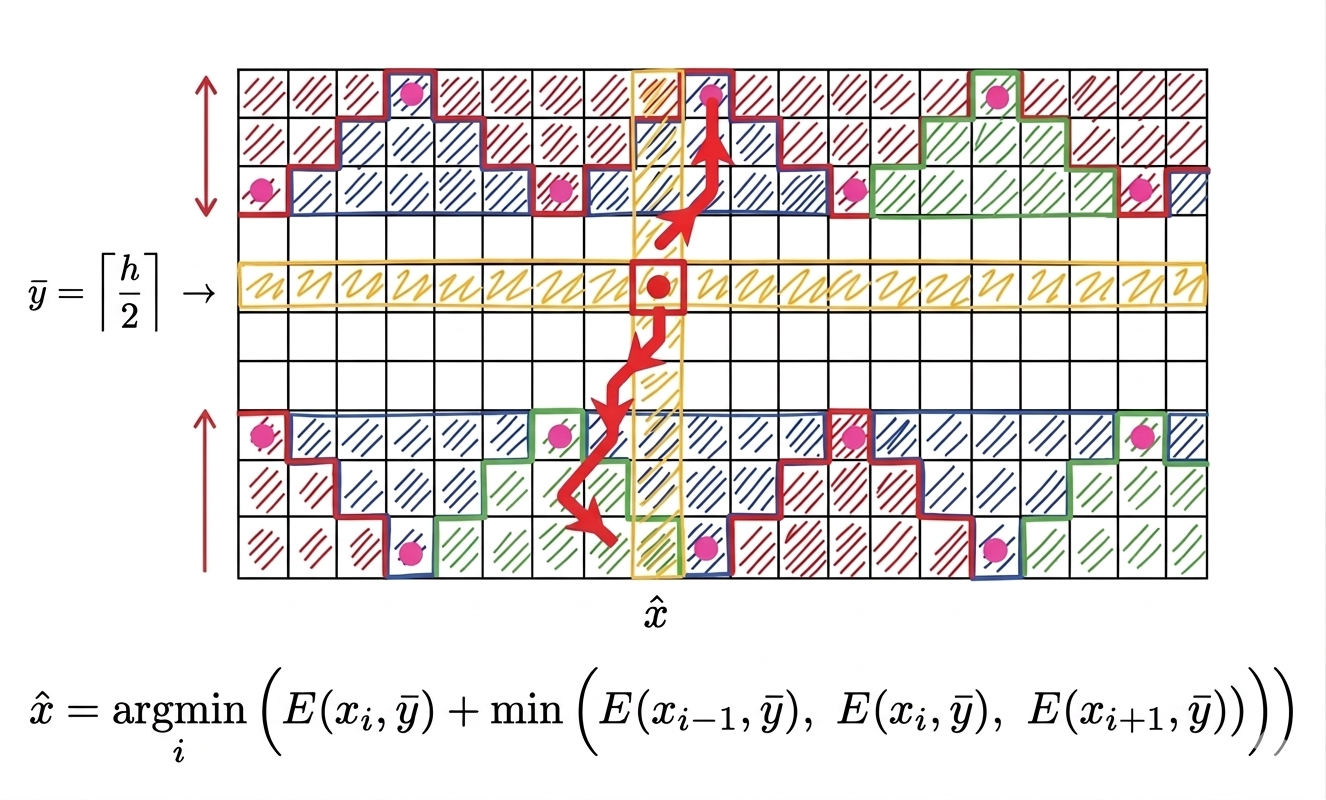
\includegraphics[width=10cm]{./images/IMG_0035.png} }}%
    \hspace{-0.4cm} 
    \subfloat[\centering Performance Results]{{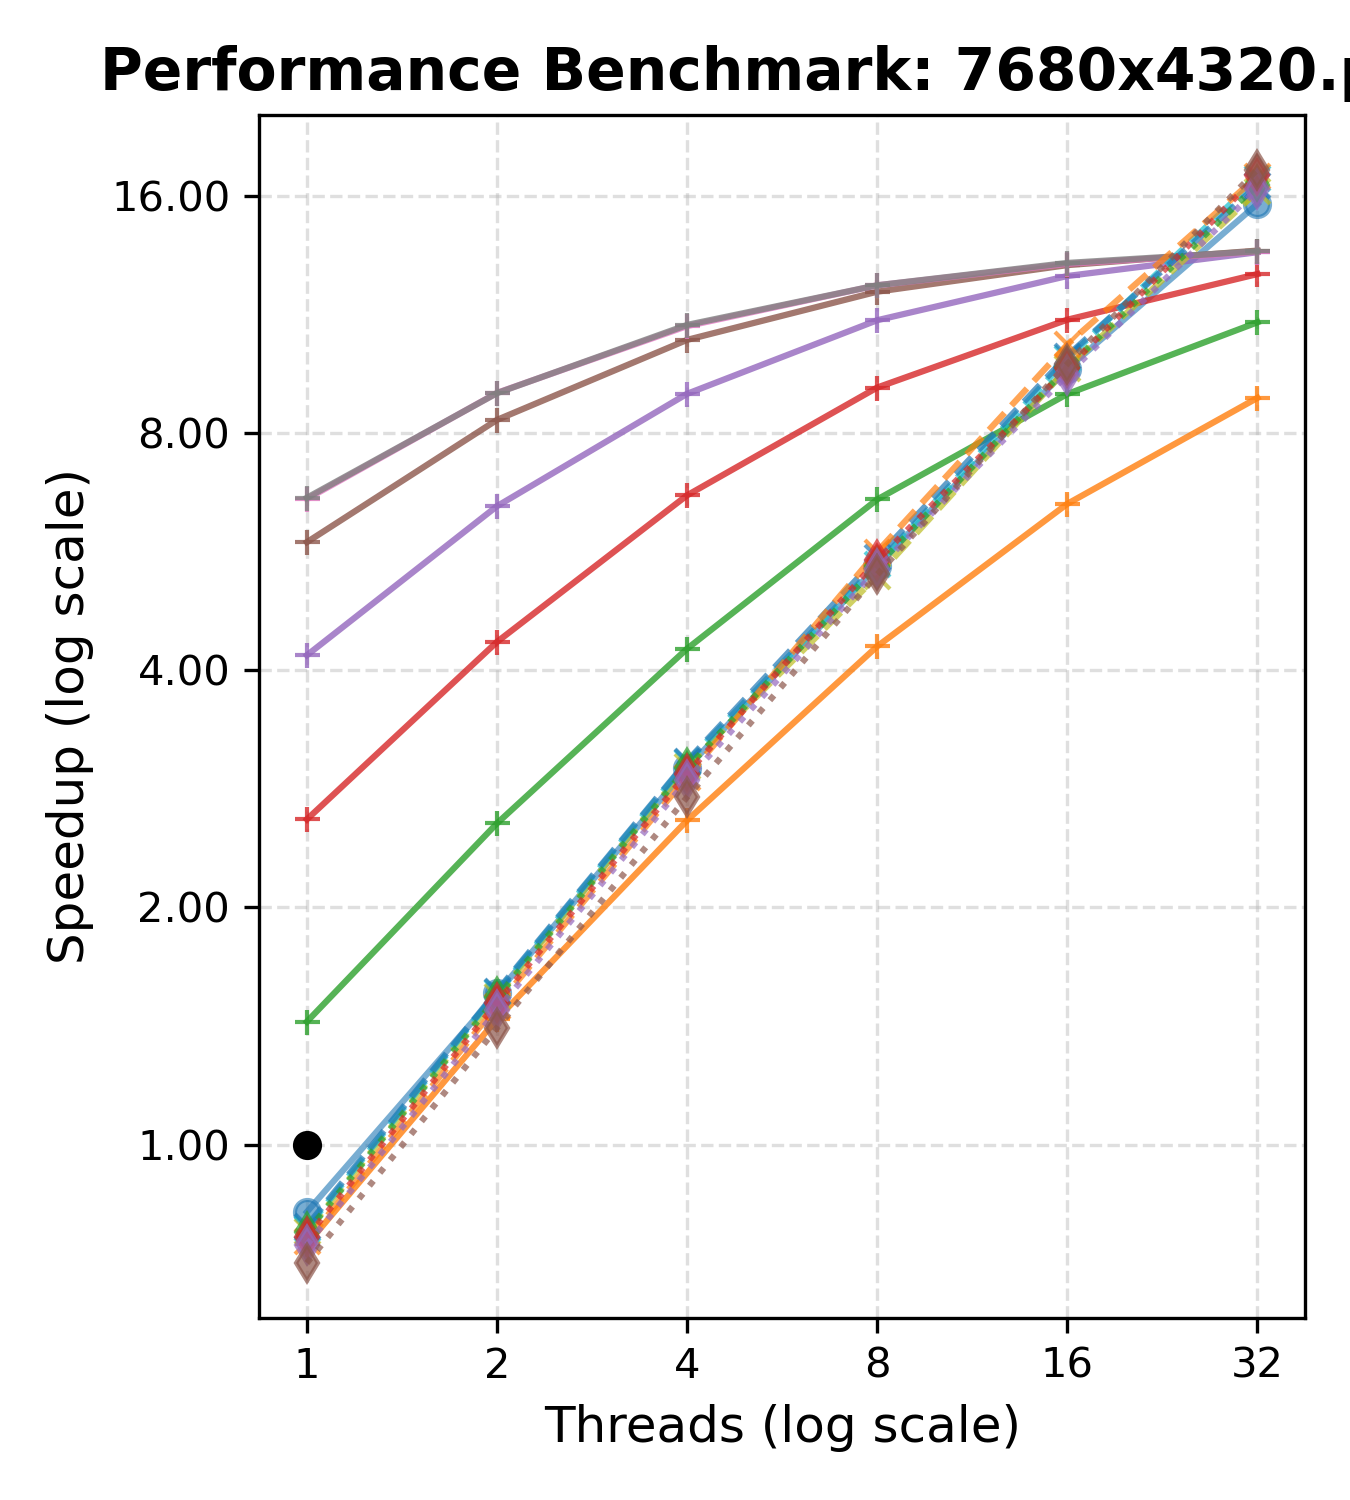
\includegraphics[width=5cm]{./images/performance_last_image.png} }}%
    \caption{Bidirectional seam carving: The left image visualizes the wavefront convergence at the midpoint $\bar{y}$, where the optimal transition point $\hat{x}$ is determined by minimizing the combined energy from both computed halves. The right image shows the corresponding performance speedup.}%
    \label{fig:midpoint_sync_comparison}%
\end{figure}



As shown in Figure \ref{fig:fixed_cores_performance}, the performance of this approach has proven effective for different cores. Specficially, for the case where the number of cores is 32 we surpass any other implementation: 





\end{enumerate}

\pagebreak 

\section{Additional data and comments:}

\begin{enumerate}
  \item   For implementing the trinagle strategy approach, we compared two tiling strategies:
  \begin{enumerate}
      \item \textbf{Case 1 ($Y \pm 1$):} The tiles have a horizontal tip of two blocks. This approach present the pink dots not uniformly distributed, see Figure \ref{fig:tiling_strategies}a). 
      
      \item \textbf{Case 2 ($Y \pm 2$):} The tiles have a single-block tip. This approach present the pink dots uniformly distributed, see Figure \ref{fig:tiling_strategies}b). 
  \end{enumerate}

  \begin{figure}[h]
      \centering
      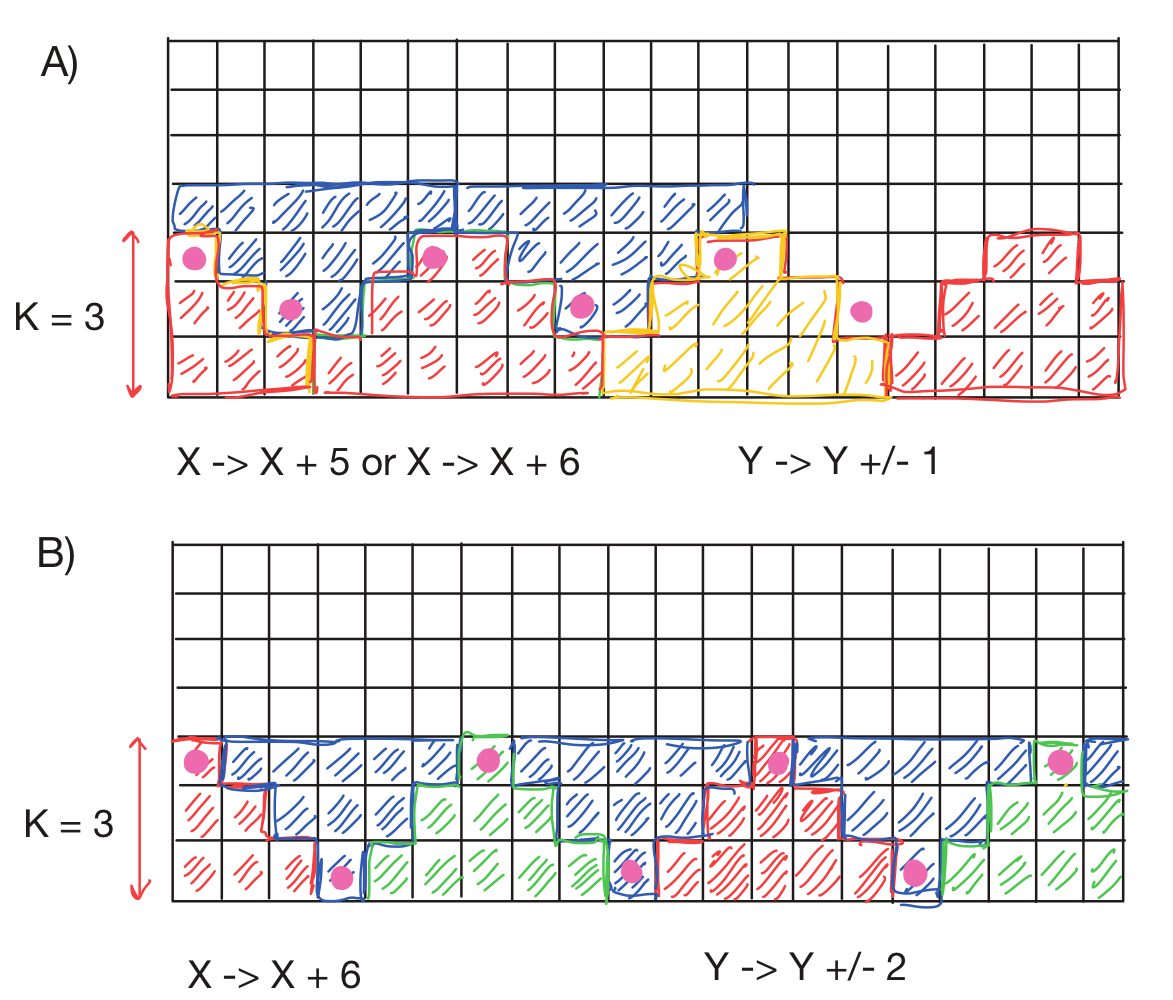
\includegraphics[width=0.65\textwidth]{./images/Imagen JPEG-482A-803F-04-0.jpeg}
      \caption{Comparison of wavefront tiling strategies for parallel seam carving for a tile height of $3$. }
      \label{fig:tiling_strategies}
  \end{figure}

  \begin{figure}[h]
        \centering
        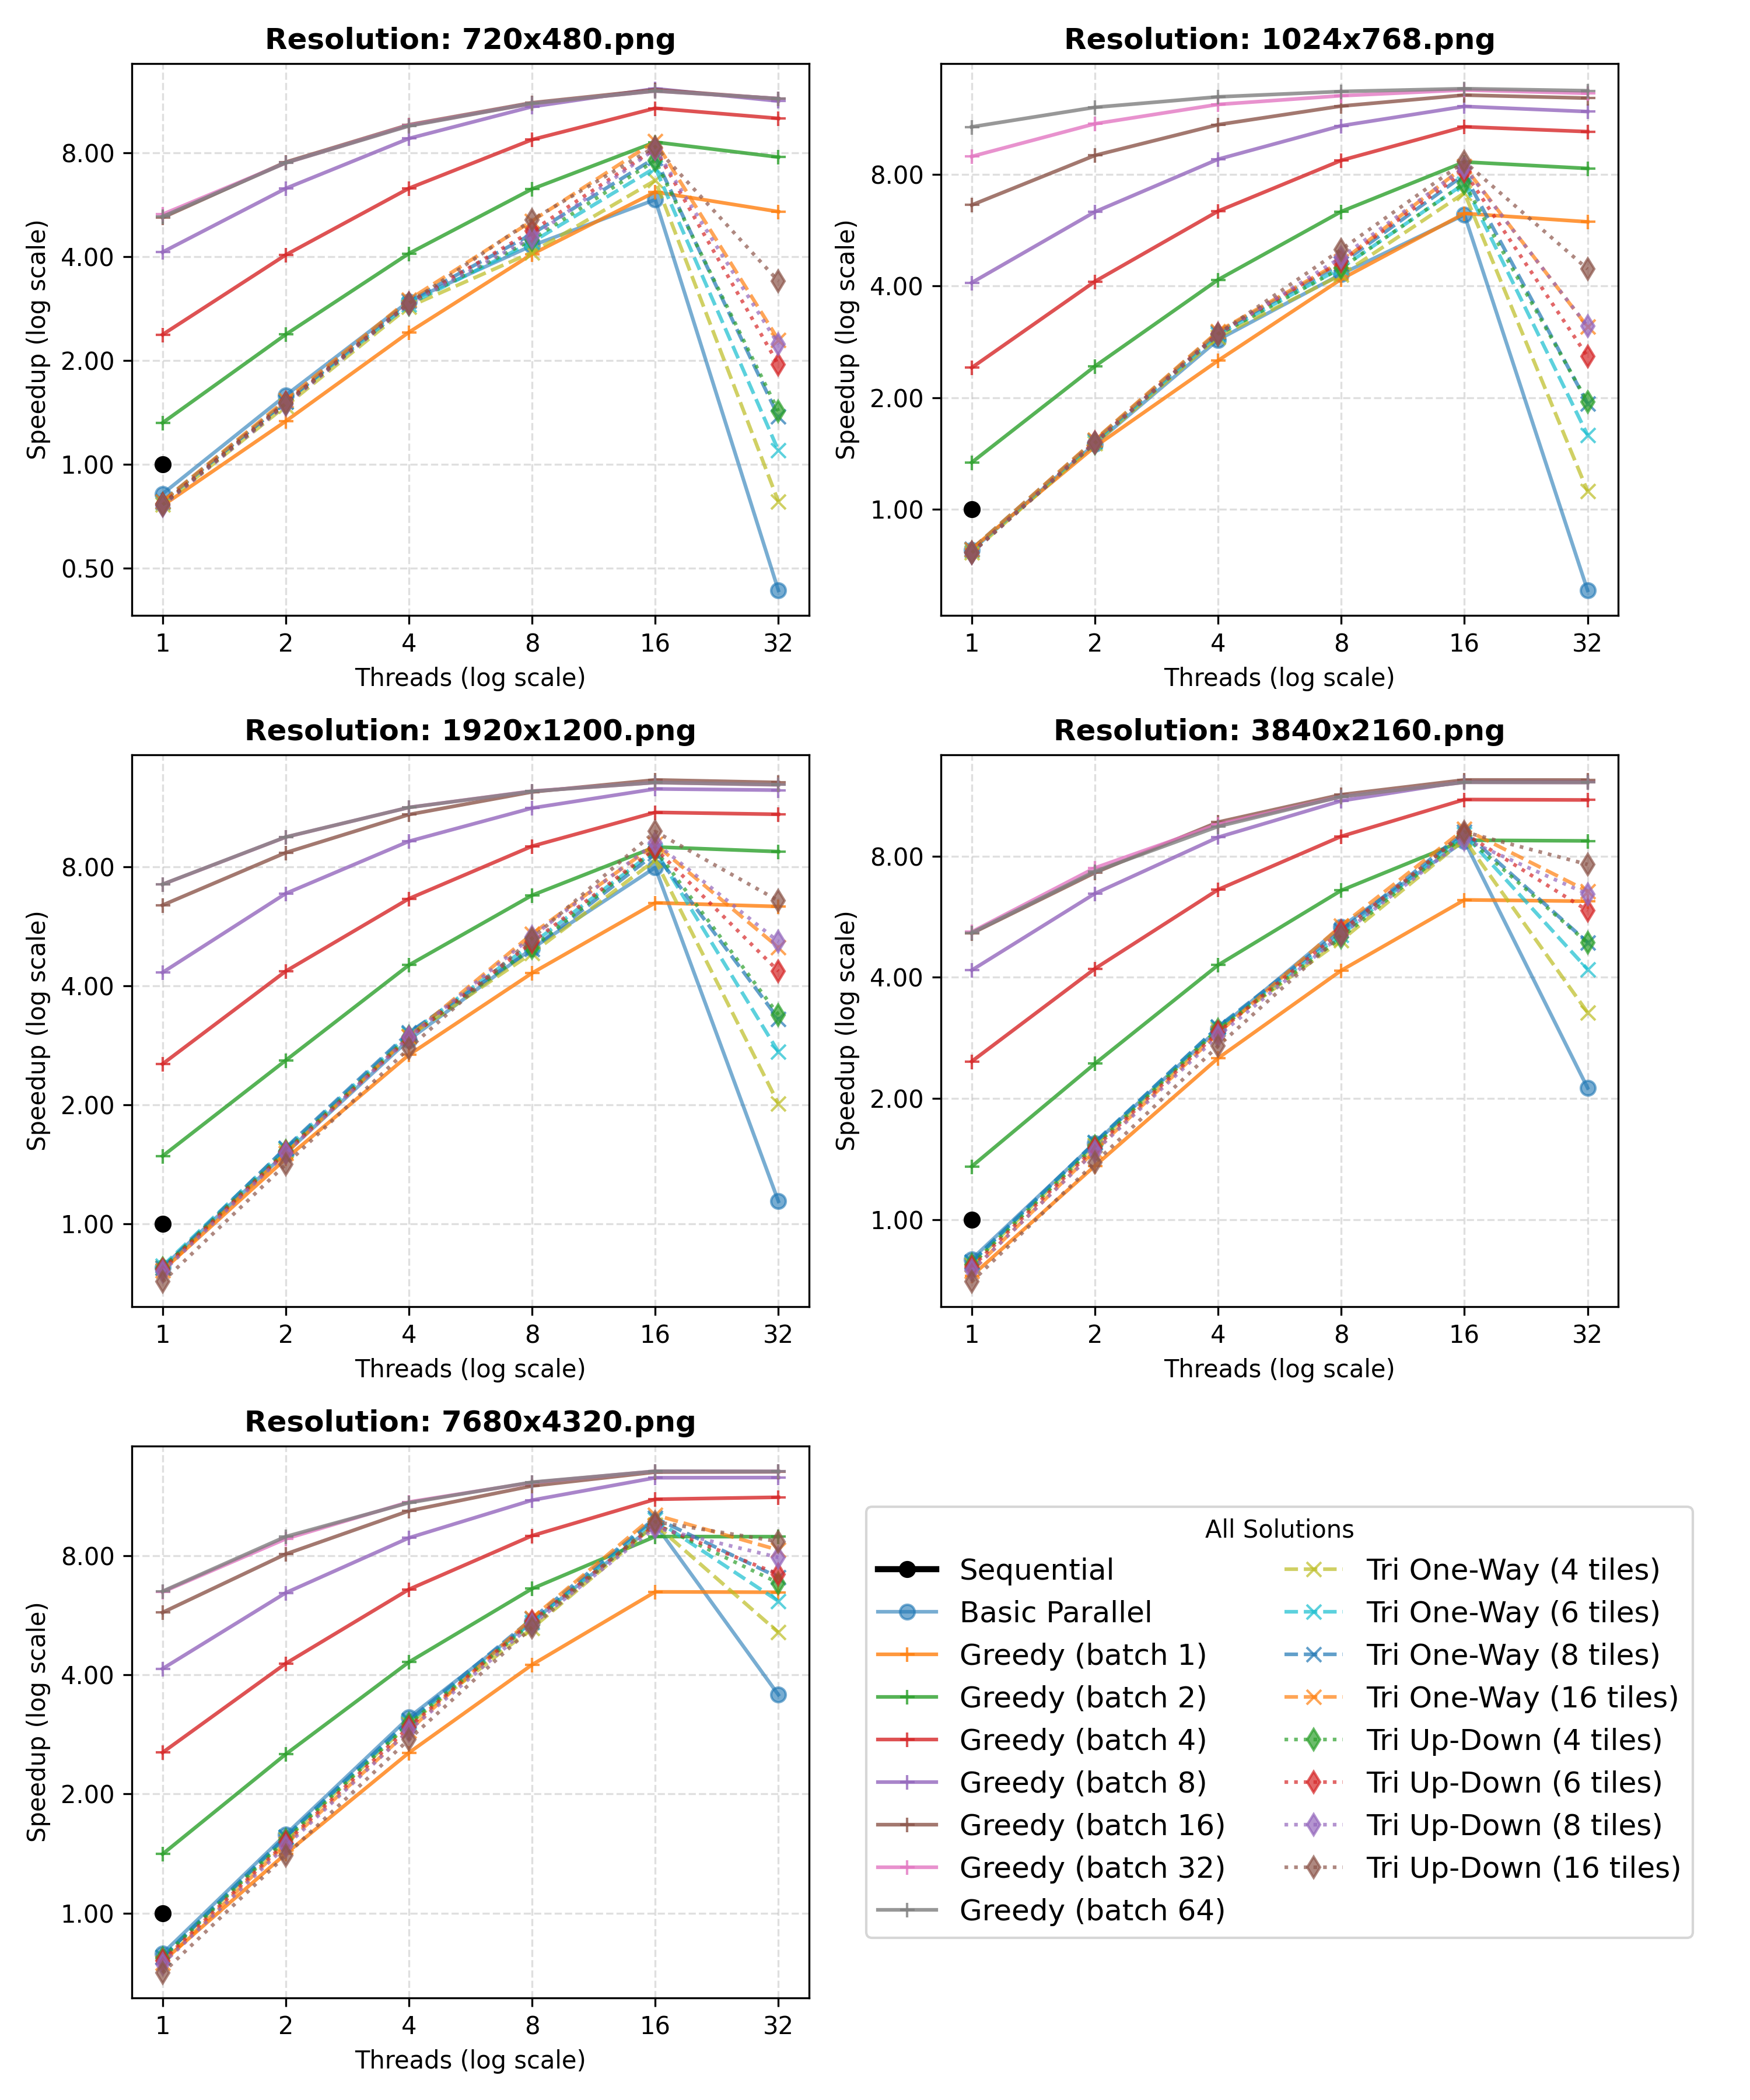
\includegraphics[width=0.8\textwidth]{./images/performance_comprehensive_greedy_16cores.png}
        \caption{Speedup analysis for various parallel strategies across five image resolutions. Case use of 16 cores.}
        \label{fig:midpoint_sync_16}
  \end{figure}

  \begin{figure}[h]
        \centering
        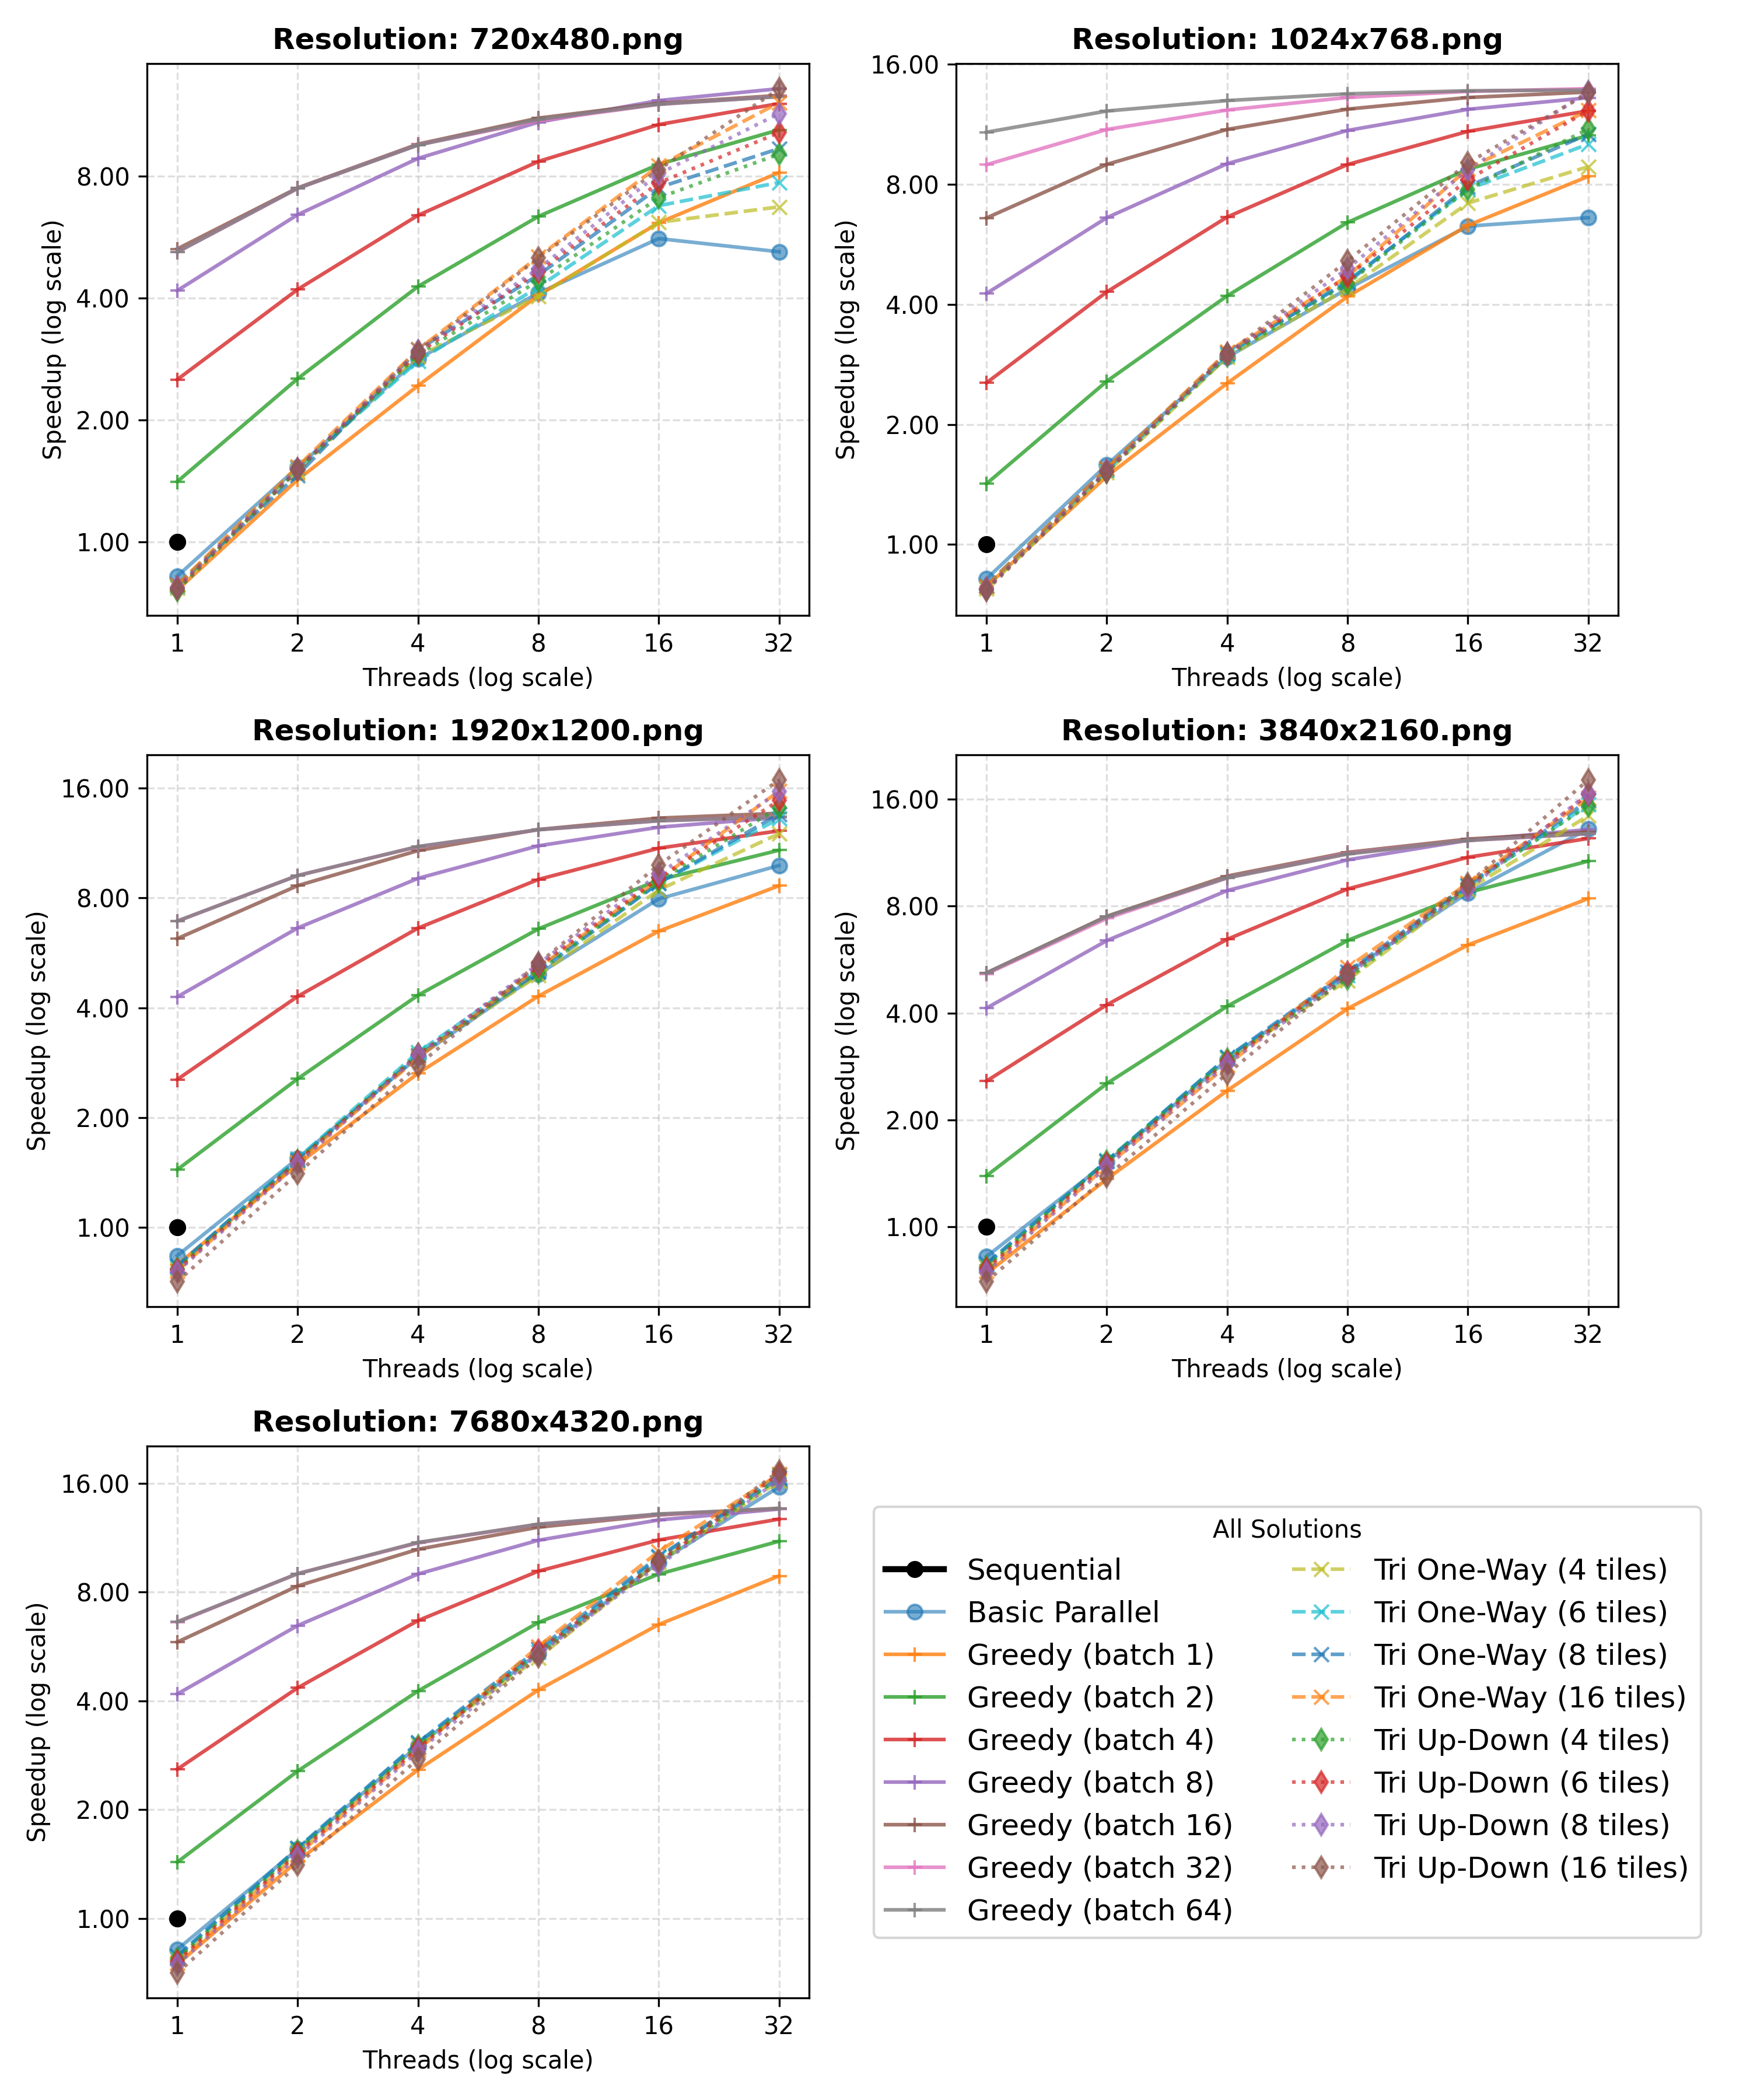
\includegraphics[width=0.8\textwidth]{./images/performance_comprehensive_greedy_32cores.png}
        \caption{Speedup analysis for various parallel strategies across five image resolutions. Case use of 32 cores.}
        \label{fig:midpoint_sync_32}
  \end{figure}


  Computationally, both options present similar performance. However, in this study the second approach (single-block tip) seems more suitable because when the height of the triangle is $k=1$, we fully return to the standard sequential approach, and, hence, we have a robust baseline to compare. 

\end{enumerate}

\end{enumerate}

\end{document}